\documentclass[UTF8]{ctexart}
\usepackage{amsmath}
\usepackage{ltablex}
\usepackage{tabularx}
\usepackage{forloop}
\usepackage{xstring}
\usepackage{ifthen}
\usepackage{calc}
\usepackage{color}
\usepackage[margin=1in]{geometry}

% \usepackage{hyperref}
% \hypersetup{pdftex,colorlinks=true,allcolors=blue}
% \usepackage{hypcap}

% \usepackage{xcolor}
\usepackage[]{hyperref}
\hypersetup{
    pdftitle={FSI Cantonese - new format},
    pdfauthor={Foreign Services Institute},
    pdfsubject={FSI Cantonese},
    bookmarksnumbered=true,
    bookmarksopen=true,
    bookmarksopenlevel=1,
    colorlinks=true,
    urlcolor=blue,
    linkcolor=black,
    pdfstartview=Fit,
    pdfpagemode=UseOutlines,
    pdfpagelayout=TwoPageRight
}

% Make font larger
\setCJKmainfont[Scale=1.5]{STSong}

% Include custom functions

%%%%%%%%%%%%%%%%%%%%%%%%%%%%%%%%%%%%%%%%%%%%%%%%%%%%%%%%%%%%%%%%%%%%%%%%%%%%%%%%

% Jyutping formatting which takes as input a string like xxxxNxxxxN and produces
% a string where the N are superscripted.
% \jping{ji4gaa1}
%
% @param string of the format xxxxNxxxxN
\newcounter{jpingStart}
\newcounter{jpingEnd}
\newcounter{jpingIndex}
\newcounter{jpingLength}
\newcounter{jpingLengthPlusOne}
\newcommand{\jping}[1]{%
    % NOTE: for single use, this would work, but we need to split...
    % \StrGobbleRight{#1}{1}\textsuperscript{\StrRight{#1}{1}}%
    % Get length of text
    \StrLen{#1}[\jpingLength]%
    \setcounter{jpingLengthPlusOne}{\jpingLength + 1}%
    % Set start of text
    \setcounter{jpingStart}{1}%
    \setcounter{jpingEnd}{0}%
    % Loop over each char
    \forloop{jpingIndex}{1}{\value{jpingIndex} < \arabic{jpingLengthPlusOne}}{%
        % Get char
        \StrChar{#1}{\arabic{jpingIndex}}[\jpingChar]%
        % If numeric, then handle
        % NOTE: include 7 for high falling examples
        \IfSubStr{1234567*}{\jpingChar}{%
            \text{\textsuperscript{\jpingChar}}%
        }{%
            \text{\jpingChar}%
        }%
    }%
}%

%%%%%%%%%%%%%%%%%%%%%%%%%%%%%%%%%%%%%%%%%%%%%%%%%%%%%%%%%%%%%%%%%%%%%%%%%%%%%%%%

% Variables for dtext
\newcounter{dtextStart}
\newcounter{dtextEnd}
\newcounter{dtextIndex}
\newcounter{dtextSubWordPlusOne}
\newcounter{dtextLength}
\newcounter{dtextLengthPlusOne}
\newcounter{dtextSubWord}
\newcounter{dtextNormal}

% Double text, meaning cantonese characters on top, and jyutping ont he bottom.
% The characters and jyutping will be grouped by spaces, with punctuation
% (including chinese punctuation), correctly ignored and skipped. Uses \jping
% for each jyutping group.
%
% Test cases
% \dtext{而家 我 問 你,你 答 我。}{ji4gaa1 ngo5 man6 nei5 nei5 daap3 ngo5}\\
% \dtext{而家 我 問 你,你 答 我。X}{ji4gaa1 ngo5 man6 nei5 nei5 daap3 ngo5 w}\\
% \dtext{而家}{ji4gaa1}\\
% \dtext{而家 我 問 你,你 答 我。a}{ji4gaa1 ngo5 man6 nei5 nei5 daap3 ngo5 -}\\
% \dtext{而家 我 問 你,你 答 我。X b}{ji4gaa1 ngo5 man6 nei5 nei5 daap3 ngo5 w -}\\
% \dtext{而家}{-}\\
% \dtext{而家。。。}{ji4gaa1}\\
% \dtext{而家 我 問 你,,你 答 我。。。}{ji4gaa1 ngo5 man6 nei5 nei5 daap3 ngo5}\\
% TODO: Mode: top only, top and bottom, bottom only, top and bottom white
%
% @param cantonese characters
% @param jyutping
\newcommand{\dtext}[2]{%
    % Get length of text
    \StrLen{#1}[\dtextLength]%
    \setcounter{dtextSubWord}{0}%
    \setcounter{dtextNormal}{0}%
    \setcounter{dtextLengthPlusOne}{\dtextLength + 1}%
    % Count number of spaces
    \StrCount{#2}{ }[\dtextSpaces]
    % Set start of word
    \setcounter{dtextStart}{1}%
    \setcounter{dtextEnd}{0}%
    % Loop over each char
    \forloop{dtextIndex}{1}{\value{dtextIndex} < \arabic{dtextLengthPlusOne}}{%
        % Get char
        \StrChar{#1}{\arabic{dtextIndex}}[\dtextChar]%
        % If special, then handle
        % https://en.wikipedia.org/wiki/Chinese_punctuation
        \IfSubStr{; 。「」﹁﹂"、‧《》〈〉﹏…——~,?;,!-?}{\dtextChar}{%
            % End of word
            \StrMid{#1}{\arabic{dtextStart}}{\arabic{dtextEnd}}[\textOver]%
            \stepcounter{dtextEnd}%
            \setcounter{dtextStart}{\arabic{dtextEnd}}%
            \stepcounter{dtextStart}%
            \ifthenelse{\equal{\arabic{dtextNormal}}{\string 0}}{%
                % No characters! Just print this one and continue
            }{%
                % Add subtext
                \ifthenelse{\equal{\arabic{dtextSubWord}}{\string 0}}{%
                    % Handle first case
                    \StrCut[1]{#2}{ }{\textUnder}{\rightpart}%
                }{%
                    % Handle last case
                    \ifthenelse{\equal{\arabic{dtextSubWord}}{\dtextSpaces}}{%
                        % IF ALL LAST .... then wont be caught...
                        \StrCut[\arabic{dtextSubWord}]{#2}{ }{\leftpart}{\textUnder}%
                    }{% Handle middle case
                        \setcounter{dtextSubWordPlusOne}{\arabic{dtextSubWord} + 1}%
                        \StrBetween[\arabic{dtextSubWord},\arabic{dtextSubWordPlusOne}]{#2}{ }{ }[\textUnder]%
                    }%
                }%
                % Handle ignore
                \ifthenelse{\equal{\textUnder}{\string -}}{%
                    \text{\textOver}%
                }{%
                    $\underset{\jping{\textUnder}}{\text{\textOver}}$%
                }%
                % \text{[\textUnder][\textOver][\dtextChar]}
                \stepcounter{dtextSubWord}%
                \setcounter{dtextNormal}{0}%
            }%
            % Enable wrapping with stupid spaces...
            \ifthenelse{\equal{\dtextChar}{ }}{%
                \text{} %
            }{%
                \text{\dtextChar}%
            }%
        }{%
            % Not end of word
            \stepcounter{dtextEnd}%
            \stepcounter{dtextNormal}%
            % Handle last not being special
            \ifthenelse{\equal{\arabic{dtextIndex}}{\dtextLength}}{%
                % End of word
                \StrMid{#1}{\arabic{dtextStart}}{\arabic{dtextEnd}}[\textOver]%
                \stepcounter{dtextEnd}%
                \setcounter{dtextStart}{\arabic{dtextEnd}}%
                \stepcounter{dtextStart}%
                % Special case of single word
                \ifthenelse{\equal{\arabic{dtextSubWord}}{\string 0}}{%
                    % FIXME: lazy...
                    \StrMid{#2}{0}{9999}[\textUnder]%
                }{%
                    \StrCut[\arabic{dtextSubWord}]{#2}{ }{\leftpart}{\textUnder}%
                }%
                % Handle ignore
                \ifthenelse{\equal{\textUnder}{\string -}}{%
                    \text{\textOver}%
                }{%
                    $\underset{\jping{\textUnder}}{\text{\textOver}}$%
                }%
            }{%
            }%
        }%
    }%
}

%%%%%%%%%%%%%%%%%%%%%%%%%%%%%%%%%%%%%%%%%%%%%%%%%%%%%%%%%%%%%%%%%%%%%%%%%%%%%%%%

% Create two column, auto numbered classroom phrases, ie
% \classroomPhrases{
%   {而家踏幾呀}{ready yet}
%   {而家踏幾呀}{ready yet}
%   {\dtext{而家踏幾呀}{ji4 gaa1 daap3 gei2 aa3}}{ready yet}
% }
%
% @param array of tuples
\newcommand*{\classroomPhrases}[1]{%
    \setcounter{classroomPhraseCounter}{1}
    \relax
    \renewcommand{\arraystretch}{2}
    \noindent\begin{tabularx}{\linewidth}{l X l X}
    \classroomPhrase#1\relax\relax
    \end{tabularx}
    \renewcommand{\arraystretch}{1}
}
\newcounter{classroomPhraseCounter}
% Helper method for classroomPhrases
\newcommand{\classroomPhrase}[2]{%
    \ifx\relax#1\\\empty%
    \else%
    \noindent\arabic{classroomPhraseCounter}. & #1 & \arabic{classroomPhraseCounter}. & #2\\\relax%
    \stepcounter{classroomPhraseCounter}%
    \expandafter\classroomPhrase%
    \fi%
}

%%%%%%%%%%%%%%%%%%%%%%%%%%%%%%%%%%%%%%%%%%%%%%%%%%%%%%%%%%%%%%%%%%%%%%%%%%%%%%%%

% Create three column, auto numbered vocabulary list, ie
% \vocabularyChecklist{
%   {A}{ex}{oh}
%   {Chahn}{sur}{Chan}
%   {deimyjhyu}{ph}{Excuse me; I beg your pardon; I'm sorry}
%   {而家踏幾呀}{abc}{ready yet}
% }
%
% @param array of triples
\newcommand*{\vocabularyChecklist}[1]{%
    \setcounter{vocabularyChecklistCounter}{1}
    \relax
    \renewcommand{\arraystretch}{2}
    \noindent\begin{tabularx}{\linewidth}{r l r X}
    \vocabularyEntry#1\relax\relax\relax
    \end{tabularx}
    \renewcommand{\arraystretch}{1}
}
\newcounter{vocabularyChecklistCounter}
% Helper method for vocabularyChecklist
\newcommand{\vocabularyEntry}[3]{%
    \ifx\relax#1\\\empty%
    \else%
    \arabic{vocabularyChecklistCounter}. & #1 & #2: & #3\\\relax%
    \stepcounter{vocabularyChecklistCounter}%
    \expandafter\vocabularyEntry%
    \fi%
}

%%%%%%%%%%%%%%%%%%%%%%%%%%%%%%%%%%%%%%%%%%%%%%%%%%%%%%%%%%%%%%%%%%%%%%%%%%%%%%%%

% Create a drill
% NOTE: does not use simple nested stuff, due to ifthenelse and multicolumn
% errors on omit

% \drillExample{
%    \drillExampleEntry {T} {\dtext{李 太,早晨}{lei5 taai2 zou2san4}} {Good morning, Mrs. Lee.}
%    \drillExampleEntry {S} {\dtext{李 太,再見}{lei5 taai2 zoi3gin3}} {Goodbye, Mrs. Lee.}
% }
% \drillExample{
%    \drillExampleEntrySub {T} {\dtext{李 太,早晨}{lei5 taai2 zou2san4}} {Good morning, Mrs. Lee.} {\dtext{陳}{can4}}
%    \drillExampleEntry {S} {\dtext{陳 太,再見}{can4 taai2 zoi3gin3}} {Good morning, Mrs. Chan.}
% }
\newcommand*{\drillExample}[1]{%
    \begin{minipage}{\linewidth}
        Ex:
        \relax
        \renewcommand{\arraystretch}{2}
        \noindent\begin{tabularx}{\linewidth}{l X | l X}
        #1\relax\relax
        \end{tabularx}
        \renewcommand{\arraystretch}{1}
    \end{minipage}
}

% Example drill entry
%
% @param speaker
% @param left
% @param right
\newcommand{\drillExampleEntry}[3]{%
    #1: & #2 & #1: & #3 \\%
}%

% Example drill entry translation
%
% @param left
% @param right
\newcommand{\drillExampleEntryTrans}[2]{%
    & #1 & & #2 \\%
}%

% Example drill entry with substitution
%
% @param speaker
% @param left
% @param right
% @param substitution
\newcommand{\drillExampleEntrySub}[4]{%
    #1. & #2 & #1. & #3 \\%
    & / #4 / & & \\%
}%

% \drill{
%    \drillEntrySub {1} {\dtext{陳 太,早晨}{can4 taai2 zou2san4}} {\dtext{李 太,早晨}{lei5 taai2 zou2san4}} {\dtext{李}{lei5}}
%    \drillEntry {2} {\dtext{劉 生,早晨}{lau4 saang1 zou2san4}}{\dtext{劉 生,再見} {lau4 saang1 zoi3gin3}}
%    \drillEntryTrans {Good morning, Mr. Lau.} {}
% }
\newcommand*{\drill}[1]{%
    \renewcommand{\arraystretch}{2}
    \noindent\begin{tabularx}{\linewidth}{l l | l l}
    #1\relax\relax
    \end{tabularx}
    \renewcommand{\arraystretch}{1}
}

% Drill entry
%
% @param number
% @param left
% @param right
\newcommand{\drillEntry}[3]{%
    \IfSubStr{1234567890}{#1}{#1.}{} & #2 & \IfSubStr{1234567890}{#1}{#1.}{} & #3 \\%
}%

% Drill entry translation
%
% @param left
% @param right
\newcommand{\drillEntryTrans}[2]{%
    & #1 & & #2 \\%
}%

% Drill entry with substitution
%
% @param number
% @param left
% @param right
\newcommand{\drillEntrySub}[4]{%
    #1. & #2 & #1. & #3 \\%
    & / #4 / & & \\%
}%

\newcommand*{\convDrill}[1]{%
    \renewcommand{\arraystretch}{2}
    \noindent\begin{tabularx}{\linewidth}{l l X | l l X}
    #1\relax\relax
    \end{tabularx}
    \renewcommand{\arraystretch}{1}
}

\newcommand{\convDrillEntry}[4]{%
    \IfSubStr{1234567890}{#1}{#1.}{} & #2: & #3 & \IfSubStr{1234567890}{#1}{#1.}{} & #2: & #4 \\%
}%


%%%%%%%%%%%%%%%%%%%%%%%%%%%%%%%%%%%%%%%%%%%%%%%%%%%%%%%%%%%%%%%%%%%%%%%%%%%%%%%%

% Create an audio tag
%
% @param tape side A/B
% @param timestamp in 0:00 format
\newcommand{\audioTag}[2]{%
    #1 $\triangleright$ #2%
}%

\newcommand{\subsText}[1]{%
    /#1/%
}

%%%%%%%%%%%%%%%%%%%%%%%%%%%%%%%%%%%%%%%%%%%%%%%%%%%%%%%%%%%%%%%%%%%%%%%%%%%%%%%%

% Create a converstation
% NOTE: does not use simple nested stuff, due to ifthenelse and multicolumn
% errors on omit
%
% \conversation{
%   %
%   \convBackground{(At the beginning of class in the morning)}
%   %
%   \convExplanation{\dtext{學生}{hok6saang1}}{student}
%   %
%   \cspeaker{\dtext{學生}{hok6saang1}}
%   \cbline{\dtext{何}{ho4}}{Ho, surname}
%   \cbline{\dtext{生}{saang1}}{Mr.}
%   \cbline{\dtext{何 生}{ho4 saang1}}{Mr. Ho}
%   \cbline{\dtext{早晨}{zou2san4}}{good morning}
%   \cfline{\dtext{何 生 早晨}{ho4 saang1 zou2san4}}{Good morning, Mr. Ho.}
%   \convExplanation{\dtext{先生}{sin1saang1}}{teacher}
%   %
%   \cspeaker{\dtext{先生}{sin1saang1}}
%   \cbline{\dtext{李}{lei5}}{Lee, surname}
%   \cbline{\dtext{太}{taai2}}{Mrs.}
%   \cbline{\dtext{李 太}{lei5 taai2}}{Mrs. Lee}
%   \cfline{\dtext{李 太 早晨。}{lei5 taai2 zou2san4}}{Good morning, Mrs. Lee.}
%   %
%   \convBackground{(At the end of the day, the students are leaving class.)}
%   %
% }
% @param table rows
\newcommand*{\conversation}[1]{%
    \relax
    \renewcommand{\arraystretch}{2}
    \noindent\begin{tabularx}{\linewidth}{X | X}
    #1\relax\relax
    \end{tabularx}
    \renewcommand{\arraystretch}{1}
}

% A line for a speaker change
%
% @param speaker name
\newcommand{\cspeaker}[1]{%
    \multicolumn{2}{c}{\textbf{\underline{#1}}} \\%
}%

% A line for a double width row (background information)
%
% @param text
\newcommand{\convBackground}[1]{%
    \multicolumn{2}{c}{#1} \\%
}%

% Buildup line
%
% @param left right
\newcommand{\cbline}[2]{%
    \indent #1 & \indent #2\\%
}%

% Full conversation line after a buildup
%
% @param left right
\newcommand{\cfline}[2]{%
    #1 & #2\\%
}%

% Additional conversation line (i.e. word explanation)
%
% @param left right
\newcommand{\convExplanation}[2]{%
    \indent #1 & \indent #2\\%
}%

\newcommand*{\listeningConversation}[1]{%
    \relax
    \renewcommand{\arraystretch}{2}
    \noindent\begin{tabularx}{\linewidth}{l l}
    #1\relax\relax
    \end{tabularx}
    \renewcommand{\arraystretch}{1}
}

\newcommand{\lcEntry}[2]{%
    #1: & #2\\%
}%

%%%%%%%%%%%%%%%%%%%%%%%%%%%%%%%%%%%%%%%%%%%%%%%%%%%%%%%%%%%%%%%%%%%%%%%%%%%%%%%%

% Translater note
%
% @param text
\newcommand{\tnote}[1]{%
    \underline{Translation Note}: #1%
}

% TODO note
%
% @param text
\newcommand{\todo}[1]{%
    \textbf{\underline{TODO}}: #1%
}

\begin{document}

\title{FSI Cantonese - new format}
\author{Foreign Services Institute}

%%%%%%%%%%%%%%%%%%%%%%%%%%%%%%%%%%%%%%%%%%%%%%%%%%%%%%%%%%%%%%%%%%%%%%%%%%%%%%%%
\maketitle

%%%%%%%%%%%%%%%%%%%%%%%%%%%%%%%%%%%%%%%%%%%%%%%%%%%%%%%%%%%%%%%%%%%%%%%%%%%%%%%%
\tableofcontents

%%%%%%%%%%%%%%%%%%%%%%%%%%%%%%%%%%%%%%%%%%%%%%%%%%%%%%%%%%%%%%%%%%%%%%%%%%%%%%%%
% Misc notes
\section{Updates}

Update to this work are available for free on \href{https://github.com/cybojanek/fsi-cantonese/releases}{github}

\section{License}

This work is licensed under a Creative Commons Attribution-ShareAlike 4.0 International License. You can find the full text \href{https://creativecommons.org/licenses/by-sa/4.0/}{here}.

In brief summary, you are free to:

\begin{itemize}
	\item Share - copy and redistribute the material in any medium or format
	\item Adapt - remix, transform, and build upon the material for any purpose, even commercially.
\end{itemize}

Under the following terms:

\begin{itemize}
	\item Attribution — You must give appropriate credit, provide a link to the license, and indicate if changes were made. You may do so in any reasonable manner, but not in any way that suggests the licensor endorses you or your use.
	\item ShareAlike — If you remix, transform, or build upon the material, you must distribute your contributions under the same license as the original.
	\item No additional restrictions — You may not apply legal terms or technological measures that legally restrict others from doing anything the license permits.
\end{itemize}

\section{Translator notes}

\begin{itemize}
    \item The original FSI course, along with the accompanying audio is available \href{https://fsi-languages.yojik.eu/languages/FSI/fsi-cantonese.html}{here}.
    \item The original FSI cantonese uses yale romanization with 7 tones. This translation uses jyupting with 6 tones.
    \item This is a work in progress.
    \item Thanks to rathy, kobo-dashi, cato, and anyone else who contributed to the conversation transcripts on the cantonese dictionary \href{http://www.cantonese.sheik.co.uk/phorum/read.php?1,53361,page=1}{forums} back in 2006.
    \item Thanks to Archive.org for having an OCR \href{https://archive.org/stream/Fsi-CantoneseBasicCourse-StudentText/Fsi-CantoneseBasicCourse-Volume1-StudentText_djvu.txt}{version} of the text.
    \item Misc digitization notes are marked as \tnote{Something is different}
    \item Things left to be copied are marked as \todo{Fix this section}
\end{itemize}

% Introduction
\section{Preface}

Cantonese is the principal language of Kwangtung province in Southeast China, parts of neighboring Kwangsi province, and Hong Kong and Macau on China's south- east periphery. In addition Cantonese is spoken by ethnic Chinese in Vietnam, Cambodia, Laos, Singapore and Malaysia, with the number of speakers in Southeast Asia being between 45 and 50 million altogether. Americans of Chinese descent in the U.S. are almost entirely of Cantonese origin.

Among the many dialects of Cantonese, the prestige variety spoken in Canton is standard, by definition, and is imitated over a wide area which includes Hong Kong. It is this dialect which is represented in the two-volume FSI Cantonese Basic Course and the related tape recordings.

The course, intended to provide a syllabus for an intensive course of about 400 classroom hours in spoken Cantonese, was prepared by Elizabeth Latimore Boyle with special assistance from Pauline Ng Delbridge. The direct costs were borne by the U.St Office of Education. The Foreign Service Institute sponsored the project and underwrote the indirect costs.

The project profited considerably from the help of Cheong Kwong-yu of the National Taiwan University, who was one of the teachers in the earliest try-out of the course and who subsequently served as advisor on pronunciation and usage. Of additional help were the suggestions of Mr. Lung Sing, Cantonese instructor in the American Consulate General in Hong Kong, and the critiques of experienced instructors under Mr. Liu Ming in Hong Kong. Liu Ming, who is director of the Chinese Language Center at New Asia College, also assisted in assembling a staff to voice the text.

Professor John McCoy of Cornell read the manuscript in an early version and made helpful suggestions. Professor James E. Dew of the University of Michigan commented on the first five lessons and contributed two sections of pronunciation drills.

Miss Telia Thweatt had a unique sequence of service in the project, participating first as a student in the try-out of the course in Taipei, then as typist and general assistant for the present version. Mrs. Lily Lu prepared most of the final typescript. Linda Birkner of the FSI secretarial staff assisted in readying the camera copy for publication.

A Cantonese-English glossary appears at the end of each volume, three columns presenting respectively a romanization, the appropriate characters, and the gloss. A fourth column indicates where the item first occurs in the text. The characters for Volume I were written by Cheong Kwong-yu, and for Volume II by George Lin, Cantonese instructor at FSL.

The U.S. Information Agency cooperated by contributing recording studio time and technical personnel in Hong Kong and Taipei to make the tape recordings which accompany these volumes. N.C. Hon in Hong Kong and Y.T. Yu in Taipei were helpful both in their patience and in the care with which they made the recordings.

The Cantonese voices on the tapes are Pauline Delbridge, Chik Hon-man, Chow Wai-ming and Lung Yue-ching for the Basic Sentences and the Conversations for Listening. For the Drills, they are Cheong Kwong-yu and Ho Suk-ching. All grew up in Hong Kong with the exception of Miss Ho. Users of the tapes should be aware that Miss Ho, the female voice in all Drills in the FSI recording of this text, portrays a few deviations from the textbook standard. Particularly noticeable will be her use of [?] before [?] where [?] standard in Canton and Hong Kong.

\todo{What are those characters?}

\begin{flushright}
James R. Frith, Dean\\
School of Language Studies\\
Foreign Service Institute\\
\end{flushright}

%%%%%%%%%%%%%%%%%%%%%%%%%%%%%%%%%%%%%%%%%%%%%%%%%%%%%%%%%%%%%%%%%%%%%%%%%%%%%%%%
\newpage
\section{Introduction}

%%%%%%%%%%%%%%%%%%%%%%%%%%%%%%%%%%%%%%%%

\subsection{Scope of the text}

This Cantonese Basic Course is a course in spoken Cantonese. It uses all the basic grammatical structures of the language and a vocabulary of approximately 950 words. The subject matter of the course deals with daily life in Hong Kong. The course was designed to be taught in an intensive language program of 25-30 class hours a week. Students are expected to spend additional time outside of class listening to tapes of the lessons. There are 30 lessons in the course, and the rate of progress in an intensive class is expected to be approximately 2 lessons per week, including time for review and testing. Each lesson contains five sections: I) a Basic Conversation to be memorised, II) Notes, III) Pattern Drills, structural drills of the type in which the teacher's cue is the stimulus fer the students' response, IV) Conversations for Listening, a listening comprehension section, and V) Say it in Cantonese, English to Cantonese practice, much of it in conversational question-answer form, in which students activate what they have learned in the lesson. The early lessons in addition contain explanation and practice drills on pronunciation points, and some classroom phrases for the students to learn to respond to when used by the teacher.

%%%%%%%%%%%%%%%%%%%%%%%%%%%%%%%%%%%%%%%%

\subsection{Method of Instruction}

Ideally, but perhaps not typically, instruction is by a team consisting of a native speaking Cantonese as instructor and a native speaking American as linguist, with the instructor teaching by voicing the Cantonese sentences of the text for the students to imitate and the linguist giving explanations in English when required. A good 80-90\% of class time will then be spent with the native speaking instructor drilling the students in recitations, during which time the language in use is entirely Cantonese. Students will read the notes of each lesson outside of class, and questions they have on the text will be answered in English by the linguist during periods set aside for that purpose. Questions in English are not asked during drill sessions with the instructor. Psychologically this establishes the habit of using only Cantonese in classes with the instructor. Class time is concentrated on learning the language by imitation, repetition, and transformation, according to spoken cues. The instructor speaks at natural speed, and the students learn to comprehend and speak at the same natural speed. If there is no linguist to explain students' questions, special periods are set aside for students to ask questions of the instructor. It is recommended that the rhythm of the drills not be interrupted by questions in English.

%%%%%%%%%%%%%%%%%%%%%%%%%%%%%%%%%%%%%%%%

\subsection{Pace}

Although the course is projected as a 16 week course if studied on an intensive program, the time plan is to be viewed as a rough guide only. The number of students in the class, their language learning aptitude, their amount of previous experience with related languages, the amount of time available for outside study, the excellence of the teacher - all these are variable factors which could affect the pace of learning.

An earlier version of the course was tested out on a pilot class of five students during the summer of 1967, and the proposed pace of two lessons a week seemed about right. However the students in that course had been selected on the basis of a roughly the same language aptitude score on the Modern Language Aptitude Test, and they had all previously studied Mandarin Chinese, a closely related language. Also, the present version incorporates pronunciation practices which the earlier version did not have, and additional Conversations for Listening and Say It In Cantonese sections.

It is therefore suggested that the teacher rely on his own judgment in regard to the pace of the lessons, rather than follow a set pace rigidly. The text has been devised so that the crucial grammatical structures are covered in the first 26 lessons. By covering the first 26 lessons well students will gain a firm structural control of the spoken language. We firmly feel that confident mastery of the first 26 lessons is preferable to hesitant control of the entire text, if a choice must be made between the two. The rule of thumb should be that before going on to a new lesson students should be able to recite the old lesson's Basic Conversation fluently and with expression and should be able to do the Pattern Drills without looking at the book and without marked hesitation.

%%%%%%%%%%%%%%%%%%%%%%%%%%%%%%%%%%%%%%%%

\subsection{Objectives of the course}

The objectives of the course are to teach students to speak Standard Cantonese in the locales where Cantonese is spoken, to speak it fluently and grammatically, with acceptable pronunciation, within the scope of topics of daily life. The course was not designed to lay the groundwork for learning the written language. At the end of the course students will be able to buy things; talk on the telephone; ask and give directions; handle money; discuss events past, present, and future; make comparisons; talk about themselves and their families; tell time; order simple meals; talk with the landlord, doctor, servant, bellboy, cabdriver, waiter, sales-clerk; discuss what, when, where, why, who, how, how much. They will not be able to discuss politics or their jobs or other topics of a specialized nature.

%%%%%%%%%%%%%%%%%%%%%%%%%%%%%%%%%%%%%%%%

\subsection{Reliability of the material}

All the conversations and drills in this book were written by native Cantonese speakers working under the direction of an American linguist who specified which grammatical points to cover and what situations were required. The design of the text - what to cover, what sequence to use in introducing new material, what limits to set on vocabulary -, the write-ups of structure notes, types and layouts of pattern drills, and the contents of the English-to-Chinese translation sections, were done by the American linguist.

What we have done to handle the problem of limited structures and vocabulary is to plan the lessons so that certain topics and forms don't come up until rather late in the course. The words 'yesterday,' 'today,' and 'tomorrow,' for example, don't occur until Lesson 16. Meanwhile the student has built up the grammatical structure and vocabulary to talk fluently on some subjects which don't involve these expressions and the complexities of verb structures that are involved with time-related sentences. For this reason the present text is not appropriate for use of students whose needs are for just a few phrases of Cantonese - it takes too long from that point of view to get to some of the phrases which a tourist, for example, wants to use right away. But the student who can study hard on an intensive program for 4 months and cover at least 26 of the 30 lessons, will then speak natural -sounding and grammatical Cantonese, and will be able to cope with most daily life situations in the language.

%%%%%%%%%%%%%%%%%%%%%%%%%%%%%%%%%%%%%%%%%%%%%%%%%%%%%%%%%%%%%%%%%%%%%%%%%%%%%%%%

\subsection{Procedure}

Basic Conversation , Each lesson begins with a Basic Conversation covering a daily life situation, organised around one or more grammatical points. The conversation is presented first in build-up form, then in recapitulation .

The buildup is partly a device to isolate new words and phrases for pronunciation and identification, partly a device to enable students to gain smooth delivery and natural sentence rhythm by starting with a small segment of a sentence then progressively adding to it to build a full sentence.

The recommended procedure for the buildup is as follows: Students open their books to the new lesson and look at the English equivalents as the teacher voices the Cantonese. The teacher voices the first item six times - three times for the students to listen only, three times for them to repeat after the teacher. (The teacher may voice the items more times, but it is recommeaded that he not do less.) The teacher then moves on to the next item and repeats the same procedure. When the entire buildup has been performed this way, the students close their books, and the teacher leads them through the buildup again giving each item one time, the students this time watching the teacher and imitating his behavior both vocal and kinetic - his lip movements, facial expressions, and body gestures. If the students have particular trouble with a portion of the buildup, the teacher may give it a few more repetitions than the rest, but if the difficulty persists, he drops it for the time being and marks it to return to later. Repetitions under pressure are quite tension producing, and it works better to return to a difficult passage in a more relaxed mood.

In the recapitulation section the conversation is repeated in full sentence form. The teacher voices each sentence at least two times, with pauses after each sentence for students to repeat. The first goal is for the students to be able to say the conversation after the teacher at natural speed and with natural sentence rhythm.

Details of pronunciation are spotlighted in another section - the first goal for the conversation is sentence rhythm and natural speed.

The second goal is for the students to memorise the Basic Conversation, so they can say it independently without the teacher's model to follow, maintaining natural speed and rhythm. Students will find the tape recorder a valuable aid to memorizing. The tape recorder is tireless in furnishing a model for students to imitate, and enables them to procede at the pace best suited to their needs.

The purpose of memorizing the Basic Conversations is twofold. Memorizing situational material gives students tip-of-the-tongue command of useable Cantonese. Secondly, since the basic conversations are organized on grammatical principles, students by memoriziag the conversations will be learning the grammatical framework of the language, on which they can construct other sentences.

The second day on the lesson, when students have memorized the conversation, it is recommended that the teacher have them act out the conversational roles. Later, after moving on to a new lesson, the teacher has them act out the Basic Conversation of an earlier lesson as a form of review.

%%%%%%%%%%%%%%%%%%%%%%%%%%%%%%%%%%%%%%%%

\subsubsection{Pronunciation Practice}

In general, the Pronunciation Practices concentrate on giving limited explanation and fuller practice drills on new sounds encountered in a lesson, plus comparison drills with sounds previously learned and sometimes comparisons with American close counterparts. Instead of giving many examples, using items unknown to the students the pronunciation drills stick to examples from material they have met in the Basic Conversation or Pattern Drills. The exception to this is Lesson One, which presents am overview of all the tones, consonant initials, and vocalic finals of the language, in addition to giving an introduction to intonation and stress. Students who absorb pronunciation best thouugh mimicking the model and who find the linguistic description of sounds confusing or boring or both, should concentrate on mimicking the model and skimp or skip the explanations.

%%%%%%%%%%%%%%%%%%%%%%%%%%%%%%%%%%%%%%%%

\subsubsection{Notes}

There are two kinds of Notes - Structure (grammar) Notes and Culture Notes. These are to be read outside of class.

The structure notes summarize the structures used in the Basic Conversations and practiced in the Pattern Drills, and are for those students who want a general explanation of how the language works. The students who absorb language structures better through learning model sentences and drilling variations of the model can concentrate on the Basic Conversations and Pattern Drills, and skimp on the Structure Notes.

The Culture Notes comment on some Cantonese life patterns which differ from our own.

%%%%%%%%%%%%%%%%%%%%%%%%%%%%%%%%%%%%%%%%

\subsubsection{Pattern Drills}

There are six kinds of Pattern Drills in Cantonese Basic Course. The purpose of the drills is to make the vocabulary and sentence structures sink in and become speech habits, so that the student understands spoken Cantonese without having to translate mentally and speaks fluently and grammatically at natural speed without awkward hesitation and groping for words.

The Pattern Drills give students practice in structures and words which have been introduced in the Basic Conversations. In addition, there are other vocabulary items which appear first in the drill sections. A plus sign marks each occurrence of a new word in this section, and the English equivalent is given.

Each drill begins with an example giving a model of the teacher's cue and the students' response. Then there follow 8 to 10 problems to be done on this pattern. The teacher gives the cue, and the student responds to the new cue following the pattern set in the example. The response is thus predictable, controlled by the pattern and the cue. In the book the cues are given in the left hand column and the responses on the right, with the example above.

Students will find that going over the drills in a session with the tape reoorder before performing them in class with the teacher aids their grasp of the material and smooths their delivery. In class students look at their books to check the example for each drill, to learn what their task is. Then they perform the drill with books closed, relying on the pattern of the example sentence and the cues provided to know what to say. A drill is mastered when the student can respond to the cues promptly, smoothly, and without reference to the book.

The types of drills follow:

\paragraph{Substitution Drills}

The teacher voices a pattern sentence, then voices a word or phrase (called a cue ) to be substituted in the original sentence. The student notes the substitution cue and substitutes it in the appropriate place to make a new sentence.

\noindent Example:

\begin{quote}
T (for teacher): Good morning, Mrs. Brown. /Jones/ \\
S (for Student): Good morning, Mrs. Jones. \\
\end{quote}

\paragraph{Expansion Drills}

There are two kinds of expansion drills. One could be called a listen-and-add drill, using vocabulary and structures familiar to the students. The teaober says a word or phrase and the students repeat it. Then the teacher voices another word or phrase and the students add that word to the original utterance, expanding it. The teacher adds another cue, and the students incorporate it, and so on, making each time a progressively longer utterance.

\noindent Example:

\begin{quote}
T: Hat \\
S: Hat \\
T: Blue \\
S: Blue hat \\
T: Two \\
S: Two blue hats. \\
T: Buy \\
S: Buy two blue hats. \\
\end{quote}

This type of expansion drill is handled a little differently if it includes new vocabulary. In that case it is performed as a listen- and-repeat drill, the students echoing the teacher.

\noindent Example:

\begin{quote}
T: Hat \\
S: Hat \\
T: Blue hat \\
S: Blue hat \\
T: Two blue hats \\
S: Two blue hats \\
\end{quote}

In the second type of expansion drill the example sentence gives the model to follow and the students expand the subsequent cue sentences according to the pattern set by the example.

\noindent Example:

\begin{quote}
T: I'm not Mrs. Lee. /Chan/ \\
S: I'm not Mrs. Lee - my name ia Chan. \\
\end{quote}

\paragraph{Response Drills}

The response drills involve 1) question stimulus and answer response, or 2) statement stimulus and statement response, or 3) statement stimulus and question response.

\noindent Ex. 1:
\begin{quote}
T: Is your name Chan? /Lee/ \\
S: No, it's Lee. \\
\end{quote}

\noindent Ex. 2:
\begin{quote}
T: He speaks Cantonese. /Mandarin/ \\
S: He speaks Mandarin too. \\
\end{quote}

\noindent Ex. 3:
\begin{quote}
T: He speaks Cantonese. /Mandarin/ \\
S: Does he speak Mandarin too? \\
\end{quote}

\paragraph{Transformation Drills}

In transformation drills the students transform the grammatical form of the cue sentences from positive to negative to question, according to the pattern set in the example. A positive to negative transformation would be:

\noindent Ex:
\begin{quote}
T: Her name is Lee. \\
S: Her name isn't Lee. \\
\end{quote}

\paragraph{Combining Drills}

In combining drills the students make one long sentence from two short cue sentences, according to the pattern set in the example.

\noindent Ex:
\begin{quote}
T: It's nine o'clock. \\
We study Chinese. \\
S: We study Chinese at nine o'clock. \\
\end{quote}

\paragraph{Conversation Drills}

In conversation drills students carry on a conversation following the pattern set by the example. The book or the teacher furnishes cues to vary the content while retaining the structure.

\noindent Ex:
\begin{quote}
A: Good morning, Mrs. Lee. \\
B: Excuse ae, I'm not Mrs. Lee. My name is Chan. \\
A: Oh, excuse ae. Miss Chan. \\
B: That's all right. \\
\\
A: ... Miss Smith. $\rightarrow$ A. Good morning. Miss Smith. \\
B: ... Brown. $\rightarrow$ B. Excuse me, I'm not Miss Smith, My name is Brown. \\
A: ... A: Oh, excuse me, Miss Brown. \\
B: ... B: That's all right.\\
\end{quote}

%%%%%%%%%%%%%%%%%%%%%%%%%%%%%%%%%%%%%%%%

\subsubsection{Conversations for Listening}

The \underline{Conversations for Listening}, recorded on tapes, give the students a chance to listen to further conversations using the vocabulary and sentence patterns of the lesson under study. These can he listened to outside of class and replayed in class, with the teacher then asking questions (in Cantonese of course) on the selections and the students answering. Usually several replays are needed before the students' comprehension of the conversation is complete. After they understand a conversation in its entirety, it is recommended that they play it through two or three more times, listening especially for the expressive elements of intonation and final particles, as these occur primarily in conversation and not as natural features of pattern sentences which the students practice -in the drill sections.

After Lesson 10, there will be new vocabulary in the Conversations for Listening, to help the story along. These words and phrases are glossed in Cantonese and English at the foot of each conversation in the printed text, but students will not be held responsible for learning them.

%%%%%%%%%%%%%%%%%%%%%%%%%%%%%%%%%%%%%%%%

\subsubsection{Say It in Cantonese}

The \underline{Say It in Cantonese} section gives situations and sentences in English, and students are to give Cantonese equivalents. This section is to be performed in class for the linguist or the teacher, though the students may prepare it beforehand if they like. Students should recognize that there is often more than one acceptable way to 'say it in Cantonese'.

%%%%%%%%%%%%%%%%%%%%%%%%%%%%%%%%%%%%%%%%

\subsubsection{Vocabulary Checklist}

At the end of each lesson is a vocabulary checklist, giving the new vocabulary for that lesson, the part of speech for each entry (noun, verb, etc.), and the English translation.

%%%%%%%%%%%%%%%%%%%%%%%%%%%%%%%%%%%%%%%%%%%%%%%%%%%%%%%%%%%%%%%%%%%%%%%%%%%%%%%%
\subsection{Suggestions for Further Practice}

The Say it in Cantonese section is the final working section of each lesson. After doing that section the teacher is encouraged to allow time for the students to carry on conversation practice using the material in the lesson. The teacher should be referee for this part, and make sure all students get a chance to participate. Some students are by nature more talkative than others, and the teacher must see to it, by asking a few questions of the more retiring students, that participation in free conversation is fairly evenly distributed and that the naturally talkative students don't do all the talking.

Repeating the dialogue of the Basic Conversations of earlier lessons is a good way to keep those vocabularies and sentences fresh in the students' minds. Also, selections from earlier dialogues can often be used during free conversation practice of the lesson under study.

%%%%%%%%%%%%%%%%%%%%%%%%%%%%%%%%%%%%%%%%%%%%%%%%%%%%%%%%%%%%%%%%%%%%%%%%%%%%%%%%
\subsection{System of Romanization Used}

The system of romanization used in the text is a modification of the Huang-Kok Yale romanization. It is described in detail in Lesson 1. In comparing Cantonese and Mandarin sentence structures the system of romanization used for the Mandarin is Yale romanization.

%%%%%%%%%%%%%%%%%%%%%%%%%%%%%%%%%%%%%%%%%%%%%%%%%%%%%%%%%%%%%%%%%%%%%%%%%%%%%%%%

\subsection{Symbols Used in This Text}

\begin{tabularx}{\linewidth}{l l}
    adj & adjective \\
    adj.s. & adjective suffix \\
    adv & adverb \\
    Aux V & auxiliary verb \\
    bf & boundform, boundword \\
    Cj & conjunction \\
    CoV & co-verb \\
    ex & exclamation; example \\
    lit. & literally \\
    m, M & measure \\
    MA & moveable adverb \\
    n, N & noun \\
    NP & noun phrase \\
    nu & number \\
    P & predicate \\
    PAdv & paired adverb \\
    PCj & paired conjunction \\
    Ph & phrase \\
    PhF & phrase frame \\
    PW & placeword \\
    prep & preposition \\
    pro & pronoun \\
    QV & quod vide (Latin for 'which see') \\
    QW & question word \\
    S & subject \\
    sp & specifier \\
    SPr & sentence prefix \\
    SP & subject-predicate sentence \\
    SVO & subject-verb-object sentence \\
    ss & sentence suffix \\
    sen.suf. & sentence suffix \\
    sur & surname \\
    t & title \\
    TA & term of address \\
    TW & timeword \\
    v, V & verb \\
    VO & verb-object construction \\
    VP & verb phrase \\
    Vsuf & verb suffix \\
    var & variant \\
    (\_) & = doesn't occur \\
    % NOTE: braces needed to prevent syntax error
    {[ ]} & 1. \underline{re}pronunciation = phonetic transcription \\
     & 2. in cumulative vocabulary list, following nount enteries = M for the N \\
     & 3. within the text of English gloss = literal tranlation of the Cantonese term \\
\end{tabularx}


% Lesson 01
\newpage
\section{Lesson 1}

\subsection{Classroom Phrases}

\audioTag{A}{0:05}

The instructor will address you in Cantonese from the first day of class. The following are some instructions which you should learn to respond to. Look at your books while the instructor reads the phrases the first time. Then close your books, and the teacher will give the phrases several more times, using gestures to help you understand. Repease the phrases after him, mimicking his movements as well as his voice, to help you absorb the rhythm and meaning.

\classroomPhrases{
	{\dtext{而家 你哋 聽住 我 講。}{ji4gaa1 nei5dei6 teng1zyu6 ngo5 gong2}}{Now you (plu.) listen while I speak. (i.e., listen, but you don't repeat)}
	{\dtext{而家 我 講,你哋 跟住 我 講。}{ji4gaa1 ngo5 gong2 nei5dei6 gan1zyu6 ngo5 gong2}}{Now I'll speak and you repeat after me.}
	{\dtext{x 本書,x 啲書。}{? bun2syu1, ? di1syu1}}{Close the book, close the books.}
	{\dtext{打開 本 書, 打開 啲 書。}{daa2hoi1 bun2 syu1, daa2hoi1 di1 syu1}}{Close the book, close the books.}
	{\dtext{而家 一 個 一 個 講。}{ji4gaa1 jat1 go3 jat1 go3 gong2}}{Now recite one by one.}
	{\dtext{一齊 講。}{jat1cai4 gong2}}{Recite all together.}
	{\dtext{而家 一齊 跟住 我 講。}{ji4gaa1 jat1cai4 gan1zyu6 ngo5 gong2}}{Now all together repeat after me.}
	{\dtext{再 講 一 次。}{zoi3 gong2 jat1 ci3}}{Say it again.}
	{\dtext{唔好 睇 書。}{m4hou2 tai2 syu1}}{Don't look at your book(s).}
}
\subsection{Basic Conversation}

\audioTag{A}{1:43}

%%%%%%%%%%%%%%%%%%%%%%%%%%%%%%%%%%%%%%%%
\subsubsection{Buildup}

\conversation{
    %
    \convBackground{(At the beginning of class in the morning)}
    %
    \convExplanation{\atext{學生}}{student}
    %
    \cspeaker{\atext{學生}}
    \cbline{\atext{何}}{Ho, surname}
    \cbline{\atext{生}}{Mr.}
    \cbline{\atext{何 生}}{Mr. Ho}
    \cbline{\atext{早晨}}{good morning}
    \cfline{\atext{何 生 早晨}}{Good morning, Mr. Ho.}
    \convExplanation{\atext{先生}}{teacher}
    %
    \cspeaker{\atext{先生}}
    \cbline{\atext{李}}{Lee, surname}
    \cbline{\atext{太}}{Mrs.}
    \cbline{\atext{李 太}}{Mrs. Lee}
    \cfline{\atext{李 太 早晨。}}{Good morning, Mrs. Lee.}
    %
    \cspeaker{\atext{學生}}
    \cbline{\atext{對唔住}}{excuse me}
    \cbline{\atext{我}}{I}
    \cbline{\atext{係}}{am, is, are}
    \cbline{\atext{唔}}{not}
    \cbline{\atext{唔係}}{am not, is not, are not}
    \cbline{\atext{我 唔係 李 太。}}{I'm not Mrs. Lee.}
    \cfline{\atext{對唔住,我 唔係 李 太。}}{Excuse me, I'm not Mrs. Lee.}
    %
    \cbline{\atext{姓}}{have the surname}
    \cbline{\atext{陳}}{Chan}
    \cfline{\atext{我 姓 陳。}}{My name is Chan.}
    %
    \cspeaker{\atext{先生}}
    \cbline{\atext{小姐}}{Miss; unmarried woman}
    \cbline{\atext{陳 小姐}}{Miss Chan}
    \cbline{\atext{呀}{aa3}}{Oh, Ah, a mild exclamation}
    \cfline{\atext{呀,對唔住 陳 小姐。}}{Oh, excuse me, Miss Chan.}
    %
    \cspeaker{\atext{學生}}
    \cfline{\atext{唔緊要}}{That's all right. \underline{OR} It doesn't matter.}
    %
    \convBackground{(At the end of the day, the students are leaving class.)}
    %
    \cspeaker{\atext{學生}}
    \cfline{\atext{再見}}{Goodbye.}
    %
    \cspeaker{\atext{先生}}
    \cfline{\atext{再見}}{Goodbye.}
}

%%%%%%%%%%%%%%%%%%%%%%%%%%%%%%%%%%%%%%%%
\subsubsection{Recapitulation}

\audioTag{A}{7:30}

\conversation{
    %
    \convBackground{(At the beginning of class in the morning)}
    %
    \cspeaker{\atext{學生}}
    \cfline{\atext{何 生 早晨}}{Good morning, Mr. Ho.}
    %
    \cspeaker{\atext{先生}}
    \cfline{\atext{李 太 早晨。}}{Good morning, Mrs. Lee.}
    %
    \cspeaker{\atext{學生}}
    \cfline{\atext{對唔住,我 唔係 李 太。}}{Excuse me, I'm not Mrs. Lee.}
    %
    \cfline{\atext{我 姓 陳。}}{My name is Chan.}
    %
    \cspeaker{\atext{先生}}
    \cfline{\atext{呀,對唔住 陳 小姐。}}{Oh, excuse me, Miss Chan.}
    %
    \cspeaker{\atext{學生}}
    \cfline{\atext{唔緊要}}{That's all right. \underline{OR} It doesn't matter.}
    %
    \convBackground{(At the end of the day, the students are leaving class.)}
    %
    \cspeaker{\atext{學生}}
    \cfline{\atext{再見}}{Goodbye.}
    %
    \cspeaker{\atext{先生}}
    \cfline{\atext{再見}}{Goodbye.}
}

\subsection{Introduction to pronunciation}
\subsubsection{Tones}

You have probably heard that Chinese languages are tone languages, and know this means that sounds which are the same except for rise and fall of the voice mean different things. This somtimes leads to confusion and/or merriment when a foreigner gets a tone wrong in a phrase, and says 'lazy' when he means 'broken', 'sugar' when he means 'soup', 'ghost' when he means 'cupboard', and so on.

\tnote{The textbook uses 7 yale tones, but in jyutping there are only really 6. The 7 is going to be used to denote the examples in this section of the high falling tone, which in jyutping is now just 1 (high level).}

\begin{minipage}{\linewidth}
In Cantonese there are seven tones, that is seven variations in voice pitch having the power to combine with an otherwise identitcal syllable to make seven different meanings. This is best illustrated by examples, which your teacher will read to you:

\audioTag{A}{9:10}

\renewcommand{\arraystretch}{2}
\begin{tabularx}{\linewidth}{l l l r}
    \jping{si7} & 思 & think & (High falling tone) \\
    \jping{si2} & 史 & history & (High rising tone) \\
    \jping{si3} & 試 & try & (Mid level tone) \\
    \jping{si1} & 詩 & poem & (High level tone) \\
    \jping{si4} & 時 & time & (Low falling tone) \\
    \jping{si5} & 市 & market & (Low rising tone) \\
    \jping{si6} & 事 & a matter; business & (Low level tone) \\
\end{tabularx}
\renewcommand{\arraystretch}{1}
\end{minipage}

Below is a practice exercise on the seven tones. Close your books and concentrate on listening to the teacher or tape. Repeate loud and clear during the pause after each syllabe or group of sylables.

\audioTag{A}{9:27}

(This practice section on the basic tones was prepared by Prof. James E. Dew).

\todo{copy practice exercises}

%%%%%%%%%%%%%%%%%%%%%%%%%%%%%%%%%%%%%%%%
\begin{minipage}{\linewidth}

\paragraph{Discussion of Tones}

There are seven tones in Standard Cantonese. Their desginations together with examples of each tone, are:

\audioTag{A}{14:36}

\renewcommand{\arraystretch}{2}
\begin{tabularx}{\linewidth}{l l l l}
    \jping{si1} & 詩 & \jping{fan1} & 分 \\
    \jping{si7} & 思 & \jping{fan7} & 婚 \\
    \jping{si2} & 史 & \jping{fan2} & 粉 \\
    \jping{si3} & 試 & \jping{fan3} & 訓 \\
    \jping{si4} & 時 & \jping{fan4} & 墳 \\
    \jping{si5} & 市 & \jping{fan5} & 憤 \\
    \jping{si6} & 事 & \jping{fan6} & 份 \\
\end{tabularx}
\renewcommand{\arraystretch}{1}

You will note that the tones have three conotours - level, rising, and falling.

There are three level tones: high level, mid level, and low level.

\audioTag{A}{15:03}

\renewcommand{\arraystretch}{2}
\begin{tabularx}{\linewidth}{l l l}
    hl: & \jping{si1} & 詩 \\
    ml: & \jping{si3} & 試 \\
    ll: & \jping{si6} & 事 \\
\end{tabularx}
\renewcommand{\arraystretch}{1}

There are two rising tones: high rising and low rising.

\audioTag{A}{15:10}

\renewcommand{\arraystretch}{2}
\begin{tabularx}{\linewidth}{l l l}
    hr: & \jping{si2} & 史 \\
    lr: & \jping{si5} & 市 \\
\end{tabularx}
\renewcommand{\arraystretch}{1}

There are two falling tones: high falling and low falling.

\audioTag{A}{15:16}

\renewcommand{\arraystretch}{2}
\begin{tabularx}{\linewidth}{l l l l}
    hf: & \jping{si7} & 思 \\
    lf: & \jping{si4} & 時 \\
\end{tabularx}
\renewcommand{\arraystretch}{1}

\end{minipage}

\begin{minipage}{\linewidth}

Following a chart devised by Y. R. Chao, we graph the tones of Cantonese on a scale of one to five, thus:

\audioTag{A}{15:26}

\centering
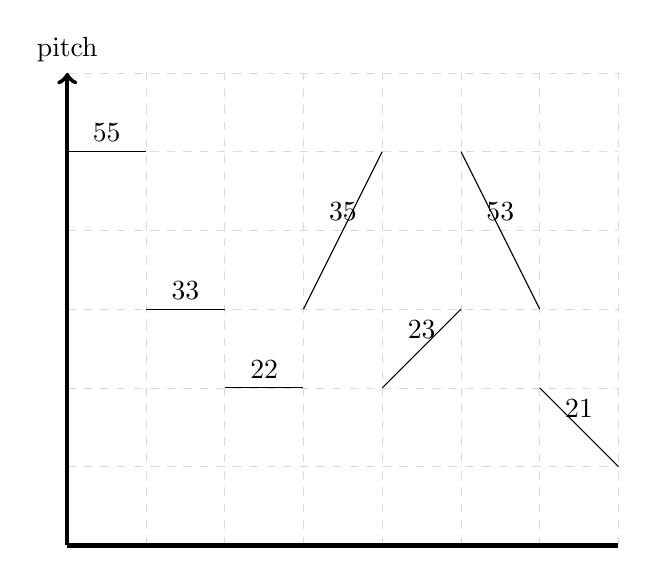
\begin{tikzpicture}
\draw [help lines, color=gray!30, dashed] (0, 0) grid (7, 6);
\draw [->, ultra thick] (0, 0) -- (0, 6) node [above]{pitch};
\draw [ultra thick] (0, 0) -- (7, 0);
\draw (0, 5) -- node [above]{55} (1, 5);
\draw (1, 3) -- node [above]{33} (2, 3);
\draw (2, 2) -- node [above]{22} (3, 2);
\draw (3, 3) -- node [above]{35} (4, 5);
\draw (4, 2) -- node [above]{23} (5, 3);
\draw (5, 5) -- node [above]{53} (6, 3);
\draw (6, 2) -- node [above]{21} (7, 1);
\end{tikzpicture}

\renewcommand{\arraystretch}{2}
\begin{tabularx}{\linewidth}{l l l l}
    high level & :55 & \jping{si1} & 詩 \\
    mid level & :33 & \jping{si3} & 試 \\
    low level & :22 & \jping{si6} & 事 \\
    high rising & :35 & \jping{si2} & 史 \\
    low rising & :23 & \jping{si5} & 市 \\
    high falling & :53 & \jping{si7} & 思 \\
    low falling & :21 & \jping{si4} & 時 \\
\end{tabularx}
\renewcommand{\arraystretch}{1}

\end{minipage}

\begin{minipage}{\linewidth}

In present day Standard Cantonese as spoken in Hong Kong the high falling tone seems to be dying out. Many people do not have a high falling tone in their speech, and use high level tones in place of high falling. These people have just six tones in their speech. In this book we mark seven tones, but your teacher may only have six, and the tapes accompanying the text include the speech of some speakers with only six tones. Copy what you hear. High falling and high level tones are given in the examples below. If you do not hear a difference, your teacher doesn't differentiate.

\audioTag{A}{15:56}

Ex: high-falling, high-level contrasts
\renewcommand{\arraystretch}{2}
\begin{tabularx}{\linewidth}{l l l l}
    1. & \jping{saam7} & three & 三 \\
       & \jping{saam1} & clothing & 衫 \\
    2. & \jping{fan7} & divide & 分 \\
       & \jping{fan1} & minute & 分 \\
    3. & \jping{ho4saang7} & Mr. Ho & 何生 \\
       & \jping{hok6saang1} & student & 學生 \\
    4. & \jping{si7} & think & 思 \\
       & \jping{si1} & poetry & 詩 \\
\end{tabularx}
\renewcommand{\arraystretch}{1}

\end{minipage}

%%%%%%%%%%%%%%%%%%%%%%%%%%%%%%%%%%%%%%%%
\begin{minipage}{\linewidth}

\paragraph{Tonal Spelling}

The system of tonal spelling we will use in this book is a modified form of the Huang-Kok yale romanization. This system divides the tones into two group, an upper register group and a lower register one. The lower register tones are marked by an \underline{h} following the vowel of the syllable. This \underline{h} is silent and simply indicates lower register. The upper register group doesn't have the \underline{h}

\audioTag{A}{16:14}

Ex: Upper register tones
\renewcommand{\arraystretch}{2}
\begin{tabularx}{\linewidth}{l l l}
    \jping{si1} & sī & 詩 \\
    \jping{si7} & sì & 思 \\
    \jping{si2} & sí & 史 \\
    \jping{si3} & si & 試 \\
\end{tabularx}
\renewcommand{\arraystretch}{1}

\audioTag{A}{16:23}

Ex: Lower register tones
\renewcommand{\arraystretch}{2}
\begin{tabularx}{\linewidth}{l l l}
    \jping{si4} & sìh & 時 \\
    \jping{si5} & síh & 市 \\
    \jping{si6} & sih & 事 \\
\end{tabularx}
\renewcommand{\arraystretch}{1}

The rising, falling, and level contours of the tones are indicated by the presence or absence of diacritics over the vowel of each syllable. The diacritics `, ´, ¯ representing falling, rising, and level respectively.

\renewcommand{\arraystretch}{2}
\begin{tabularx}{\linewidth}{l l}
    à & falling \\
    á & rising \\
    ā & level \\
\end{tabularx}
\renewcommand{\arraystretch}{1}

The absence of a diacritic represents level tone.

\renewcommand{\arraystretch}{2}
\begin{tabularx}{\linewidth}{l l}
    a & \\
\end{tabularx}
\renewcommand{\arraystretch}{1}

\end{minipage}

\begin{minipage}{\linewidth}

Using three diacritics and the low register symbol \underline{h}, we spell the seven tones thus:

\renewcommand{\arraystretch}{2}
\begin{tabularx}{\linewidth}{l l l}
    \jping{a1} & ā & high level \\
    \jping{a3} & a & mid level \\
    \jping{a6} & ah & low level \\
    \jping{a7} & à & high falling \\
    \jping{a4} & àh & low falling \\
    \jping{a2} & á & high rising \\
    \jping{a5} & áh & low rising \\
\end{tabularx}
\renewcommand{\arraystretch}{1}

\end{minipage}

\begin{minipage}{\linewidth}

The low register symbol \underline{h} follows the vowel of the syllable. If the syllable ends with a consonant, the \underline{h} still follows the vowel, but comes before the final consonant.

\audioTag{A}{16:29}

\renewcommand{\arraystretch}{2}
\begin{tabularx}{\linewidth}{l l l}
    \jping{sap6} & sahp & ten \\
    \jping{seng4} & sèhng & whole, entire \\
\end{tabularx}
\renewcommand{\arraystretch}{1}

\end{minipage}

\begin{minipage}{\linewidth}

Traditionally Chinese recite Cantonese tones in upper register - lower register sequence, in the order falling, rising, level, thus.

\audioTag{A}{16:37}

\renewcommand{\arraystretch}{2}
\begin{tabularx}{\linewidth}{l l l}
    \jping{si7} & 思 & 53 \\
    \jping{si2} & 史 & 35 \\
    \jping{si3} & 試 & 33 \\
    \jping{si4} & 時 & 21 \\
    \jping{si5} & 市 & 23 \\
    \jping{si6} & 事 & 22 \\
\end{tabularx}
\renewcommand{\arraystretch}{1}

\centering
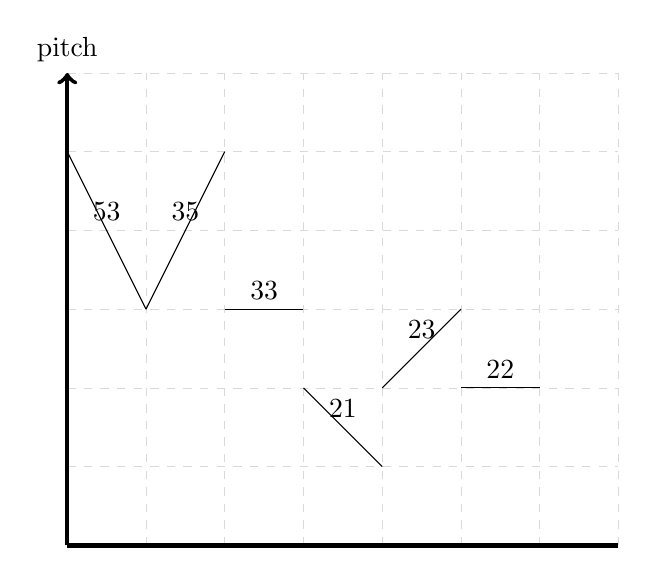
\begin{tikzpicture}
\draw [help lines, color=gray!30, dashed] (0, 0) grid (7, 6);
\draw [->, ultra thick] (0, 0) -- (0, 6) node [above]{pitch};
\draw [ultra thick] (0, 0) -- (7, 0);
\draw (0, 5) -- node [above]{53} (1, 3);
\draw (1, 3) -- node [above]{35} (2, 5);
\draw (2, 3) -- node [above]{33} (3, 3);
\draw (3, 2) -- node [above]{21} (4, 1);
\draw (4, 2) -- node [above]{23} (5, 3);
\draw (5, 2) -- node [above]{22} (6, 2);
\end{tikzpicture}

This is the way Cantonese themselves recite tones. You will note that the high level tone is not recieted traditionally. There are historical reasons for this which we won't go into here.

\end{minipage}

\begin{minipage}{\linewidth}

In a few words the consonants \underline{m} and \underline{ng} occur as vowels, and in this cases the diacritics are places above the \underline{n} of \underline{ng} and the \underline{m}.

\audioTag{A}{16:52}

\renewcommand{\arraystretch}{2}
\begin{tabularx}{\linewidth}{l l l}
    \jping{m4} & m̀h & not \\
    \jping{ng5} & ńgh & five \\
\end{tabularx}
\renewcommand{\arraystretch}{1}

\end{minipage}

%%%%%%%%%%%%%%%%%%%%%%%%%%%%%%%%%%%%%%%%
\begin{minipage}{\linewidth}

\paragraph{Tones in Sequence}

\underline{Tone Sandhi}. Changes in the basic sound of tones when syllables are spoken in sequence is called tone sandhi. The high falling tone in Cantonese undergoes tone sandhi in certain position, as follows:

\audioTag{A}{17:03}

1. When high falling tones occur in succession without intervening pause, all but the final ones are pronounced as high level:

Ex: hf + hf becomes hl + hf

\renewcommand{\arraystretch}{2}
\begin{tabularx}{\linewidth}{X X X}
roast pig (roast pork) & \dtext{燒豬}{siu7zyu7} & \dtext{燒豬}{siu1zyu7} \\
hurt wind (to catch cold) & \dtext{傷風}{soeng7fung7} & \dtext{傷風}{soeng1fung7} \\
hurt wind tim! (hurt wind!), caught cold! & \dtext{傷風添}{soeng7fung7tim7} & \dtext{傷風添}{soeng1fung1tim7} \\
\end{tabularx}
\renewcommand{\arraystretch}{1}

\audioTag{A}{17:43}

2. When a high falling tone occurs before a high level tone without intervening pause, it is pronounced as high level.

Ex: hf + hl becomes hl + hl

\renewcommand{\arraystretch}{2}
\begin{tabularx}{\linewidth}{X X X}
rent house (to rent a house) & \dtext{租屋}{zou7uk1} & \dtext{租屋}{zou1uk1} \\
west meal (western food) & \dtext{西餐}{sai7caan1} & \dtext{西餐}{sai1caan1} \\
\end{tabularx}
\renewcommand{\arraystretch}{1}

In this book high falling tone has been written high level only when the tone sandhi is within word boundaries. For separate words, the high falling will be marked with its usual diacritic.

\renewcommand{\arraystretch}{2}
\begin{tabularx}{\linewidth}{X X X}
first born (man, teacher, Mr.) & \dtext{先生}{sin7saang7} & \dtext{先生}{sin1saang7} \\
Cheung Mr. (Mr. Cheung) & \dtext{張生}{zoeng7saang7} & \dtext{張生}{zoeng7saang7} \\
\end{tabularx}
\renewcommand{\arraystretch}{1}

\end{minipage}

%%%%%%%%%%%%%%%%%%%%%%%%%%%%%%%%%%%%%%%%
\paragraph{Tones not 'sung'}

That Cantonese is a tone language does not mean that sentences in it are sung as you would sign a medical phrase. Music has sustained notes and strict rhythmic scheme, the spoken language does not. At first you may feel that Cantonese sounds sing-song, but practice will bring familiarity and soon it will sound natural to you.
\subsubsection{Intonation}

A sentence may be said different ways, to stress different points in the sentence and also to express what the speaker feels about what he is saying. To give an English example, the sentence 'So glad you could come', may be said:

\todo{contour graphs}

\begin{tabularx}{\linewidth}{X X X}
So glad you could \underline{come}. &
\begin{tikzpicture}
\draw (0, 0) -- (3, 0);
\draw (3, 0) -- (4, 0.5);
\draw [->] (4, 0.5) -- (4.5, 0);
\end{tikzpicture}
& normal polite \\

\underline{So} glad you could come. &
\begin{tikzpicture}
\draw (0, 0.5) -- (1, 0);
\draw (1, 0) -- (4, 0);
\draw [->] (4, 0) -- (4.5, -0.5);
\end{tikzpicture}
& effusive polite \\

So glad \underline{you} could come. &
\begin{tikzpicture}
\draw (0, 0) -- (1, 0);
\draw (1, 0) -- (2, 0.5);
\draw (2, 0.5) -- (3, 0);
\draw (3, 0) -- (4, 0);
\draw [->] (4, 0) -- (4.5, -0.5);
\end{tikzpicture}
& (even if your wife couldn't make it) cordial \\

So glad \underline{you} could come. &
\begin{tikzpicture}
\draw (0, 0) -- (1, 0);
\draw (1, 0) -- (2, 0.75);
\draw (2, 0.75) -- (3, 0);
\draw (3, 0) -- (4, 0);
\draw [->] (4, 0) -- (4.5, -0.5);
\end{tikzpicture}
& (even if your \underline{wife} couldn't) sarcastic \\

So glad you \underline{could} come. &
\begin{tikzpicture}
\draw (0, 0) -- (2, 0);
\draw (2, 0) -- (3, 0.5);
\draw [->] (3, 0.5) -- (4.5, -0.5);
\end{tikzpicture}
& (after having though you couldn't) cordial \\

They were glad you could come? &
\begin{tikzpicture}
\draw (0, 0) -- (4, 0);
\draw (4, 0) -- (4.5, 0.5);
\draw [->] (4.5, 0.5) -- (5, 1);
\end{tikzpicture}
& question \\
\end{tabularx}

The graphs of the sentence contours above represent the rise and fall of the voice pitch throughout the length of the sentence. This rise and fall over sentence length we call and "intonation".

You will note that the question sentence (\#5) rises in pitch at the end, and the statement sentences (\#1 - 4) all end with falling pitch, although within their contours rise and fall occurs at different points. In English sentence-final fall is the norm, and sentence-final expresses doubt.

Intonation asl has another job within a sentence, it can express how the speaker feels about what he is saying. By expressive rise and fall of his voice, by varying his "tone of voice", the speaker can indicate that he is angry or happy, doubtful or certain, being polite or rude, suggesting or demanding.

Cantonese sentences too exhbiti intonation contours. Sentence final contours in particular are much more varied in Cantonese than in English, and capable of expressing quite a range of emotional implications.

You may wonder how intonation affects the tone situation in Cantonese, each syllable having as it done its characteristic tone. How the tone contours operate in the framework of sentence contour has been compared to the action of ripples riding on top of waves. Each ripple relates to the one before it and behind it, whether in the trough of the wave or on the crest.

%%%%%%%%%%%%%%%%%%%%%%%%%%%%%%%%%%%%%%%%%%%%%%%%%%%%%%%%%%%%%%%%%%%%%%%%%%%%%%%%
\paragraph{Sentence Stress}

In speaking of sentence stress we mean relative prominence of syllables in a sentence - loud or soft (heavy or light), rapid or slow. Consider the stress pattern of the following English sentences.

\begin{tabularx}{\linewidth}{X X X}
\underline{I'm} John Smith. & (In response to "Which one of you is John Smith?") \\
I'm \underline{John} Smith. & (In response to "I was suppsed to give this letter to Tom Smith") \\
\end{tabularx}

In the sentence above the stressed syllables (those underlined) give prominence to the information requested in the stimulus sentences.

In certain sentences stress differences alone indicate dfference in message content. The pair of sentences often quoted in illustration of this is:

\begin{tabularx}{\linewidth}{X X X}
\underline{Ship} sails today. && (The ship will sail today.) \\
Ship \underline{sails} today. && (Please ship the sails today.) \\
\end{tabularx}

Another example, from a headline in a newspaper:
\indent Boy Scratching Cat is Caught, Destroyed
How do you stress that one?

%%%%%%%%%%%%%%%%%%%%%%%%%%%%%%%%%%%%%%%%%%%%%%%%%%%%%%%%%%%%%%%%%%%%%%%%%%%%%%%%
\paragraph{Sentence Pause}

Another feature important in establishing natural sentence rhythm is pause - the small silences between groups of syllables. Note the following English sentence:

\begin{quote}
	In considering him for the job he took into account his education, previous experience, and appraised potential.
\end{quote}

There is a pause between "job" and "he" in the sentence above, and if you read it instead pausing after "took", you find the sentence doesn't make sense - you have to go back and read it again putting a pause in the right place.

We will not discuss Cantonese stress and pause features in this Introduction, other than to say that Cantonese sentences, like English ones, do exhibit stress and pause phenomena, as well as intonational ones. What this effectively means for you as a student is that you must not concentrate solely on learning words as individual isolated units, but in imitating the teacher's spoken model, you should be alert to his delivery of prhase-length segments and whole sentences, and should mimic the stress, pause, and intonation of the phrases you repeat.

\subsubsection{Consonants and Vowels}
\todo{copy}

\subsection{Pronounciation Practice}
\todo{copy}
\subsection{Culture Notes}
\todo{copy}
\subsection{Drills}

%%%%%%%%%%%%%%%%%%%%%%%%%%%%%%%%%%%%%%%%

\begin{minipage}{\linewidth}

\paragraph{1. Subsitution Drill} Substitute \dtext{再見}{zoi3gin3} in the position of \dtext{早晨}{zou2san4} following the pattern of the example sentence.

\drillExample{
    \drillExampleEntry {T} {\dtext{李 太,早晨}{lei5 taai2 zou2san4}} {Good morning, Mrs. Lee.}
    \drillExampleEntry {S} {\dtext{李 太,再見}{lei5 taai2 zoi3gin3}} {Goodbye, Mrs. Lee.}
}

\drill{
    \drillEntry {1} {\dtext{陳 太,早晨}{can4 taai2 zou2san4}}{\dtext{陳 太,再見} {can4 taai2 zoi3gin3}}
    \drillEntryTrans {Good morning, Miss Chan.} {}
    %
    \drillEntry {2} {\dtext{劉 生,早晨}{lau4 saang1 zou2san4}}{\dtext{劉 生,再見} {lau4 saang1 zoi3gin3}}
    \drillEntryTrans {Good morning, Mr. Lau.} {}
    %
    \drillEntry {3} {\dtext{張 小姐,早晨}{zoeng1 siu2ze2 zou2san4}}{\dtext{張 小姐,再見} {zoeng1 siu2ze2 zoi3gin3}}
    \drillEntryTrans {Good morning, Miss Cheung.} {}
    %
    \drillEntry {4} {\dtext{馬 生,早晨}{maa5 saang1 zou2san4}}{\dtext{馬 生,再見} {maa5 saang1 zoi3gin3}}
    \drillEntryTrans {Good morning, Mr. Ma.} {}
    %
    \drillEntry {5} {\dtext{李 太,早晨}{lei5 taai2 zou2san4}}{\dtext{李 太,再見}{lei5 taai2 zoi3gin3}}
    \drillEntryTrans {Good morning, Miss Lee.} {}
}

\end{minipage}

%%%%%%%%%%%%%%%%%%%%%%%%%%%%%%%%%%%%%%%%%%%%%%%%%%%%%%%%%%%%%%%%%%%%%%%%%%%%%%%%

\begin{minipage}{\linewidth}

\paragraph{2. Subsitution Drill} Substitute the cue in the appropriate position following the pattern of the example sentence.

\drillExample{
    \drillExampleEntrySub {T} {\dtext{李 太,早晨}{lei5 taai2 zou2san4}} {Good morning, Mrs. Lee.} {\dtext{陳}{can4}}
    \drillExampleEntry {S} {\dtext{陳 太,再見}{can4 taai2 zoi3gin3}} {Good morning, Mrs. Chan.}
}

\drill{
    \drillEntrySub {1} {\dtext{陳 太,早晨}{can4 taai2 zou2san4}} {\dtext{李 太,早晨}{lei5 taai2 zou2san4}} {\dtext{李}{lei5}}
    \drillEntrySub {2} {\dtext{李 太,早晨}{lei5 taai2 zou2san4}} {\dtext{王 太,早晨}{wong4 taai2 zou2san4}} {\dtext{王}{wong4}}
    \drillEntrySub {3} {\dtext{王 太,早晨}{wong4 taai2 zou2san4}} {\dtext{何 太,早晨}{ho4 taai2 zou2san4}} {\dtext{何}{ho4}}
    \drillEntrySub {4} {\dtext{何 太,早晨}{ho4 taai2 zou2san4}} {\dtext{張 太,早晨}{zoeng1 taai2 zou2san4}} {\dtext{張}{zoeng1}}
    \drillEntrySub {5} {\dtext{劉 太,早晨}{lau4 taai2 zou2san4}} {\dtext{陳 太,早晨}{can4 taai2 zou2san4}} {\dtext{陳}{can4}}
}

\end{minipage}

%%%%%%%%%%%%%%%%%%%%%%%%%%%%%%%%%%%%%%%%%%%%%%%%%%%%%%%%%%%%%%%%%%%%%%%%%%%%%%%%

\begin{minipage}{\linewidth}

\paragraph{3. Subsitution Drill} Substitute the cue in the appropriate position, following the pattern of the example sentence.

\drillExample{
    \drillExampleEntrySub {T} {\dtext{王 生,早晨}{wong4 saang1 zou2san4}} {Good morning, Mr. Wong.} {\dtext{太}{taai2}}
    \drillExampleEntry {S} {\dtext{王 太,早晨}{wong4 taai2 zou2san4}} {Good morning, Mrs. Wong.}
}

\drill{
    \drillEntrySub {1} {\dtext{王 太,早晨}{wong4 taai2 zou2san4}} {\dtext{王 小姐,早晨}{wong4 siu2ze2 zou2san4}} {\dtext{小姐}{siu2ze2}}
    \drillEntrySub {2} {\dtext{王 小姐,早晨}{wong4 siu2ze2 zou2san4}} {\dtext{劉 小姐,早晨}{lau4 siu2ze2 zou2san4}} {\dtext{劉}{lau4}}
    \drillEntrySub {3} {\dtext{劉 小姐,早晨}{lau4 siu2ze2 zou2san4}} {\dtext{劉 小姐,再見}{lau4 siu2ze2 zoi3gin3}} {\dtext{再見}{zoi3gin3}}
    \drillEntrySub {4} {\dtext{劉 小姐,再見}{lau4 siu2ze2 zoi3gin3}} {\dtext{劉 生,再見}{lau4 saang1 zoi3gin3}} {\dtext{生}{saang1}}
    \drillEntrySub {5} {\dtext{劉 生,再見}{lau4 saang1 zoi3gin3}} {\dtext{劉 太,再見}{lau4 taai2 zoi3gin3}} {\dtext{太}{taai2}}
}

\end{minipage}

%%%%%%%%%%%%%%%%%%%%%%%%%%%%%%%%%%%%%%%%%%%%%%%%%%%%%%%%%%%%%%%%%%%%%%%%%%%%%%%%

\begin{minipage}{\linewidth}

\paragraph{4. Expansion Drill} Expand the cue sentance as indicated in the example.

\drillExample{
    \drillExampleEntry {T} {\dtext{我 唔係 王 生}{ngo5 m4hai6 wong4 saang1}} {I'm not Mr. Wong.}
    \drillExampleEntry {S} {\dtext{對唔住 我 唔係 王 生}{deoi3m4zyu6 ngo5 m4hai6 wong4 saang1}}
}

\drill{
    \drillEntry {1} {\dtext{我 唔係 李 小姐}{ngo5 m4hai6 lei5 sui2ze2}} {\dtext{對唔住,我 唔係 李 小姐}{deoi3m4zyu6 ngo5 m4hai6 lei5 sui2ze2}}
    \drillEntry {2} {\dtext{我 唔係 陳 生}{ngo5 m4hai6 can4 saang1}} {\dtext{對唔住,我 唔係 陳 生}{deoi3m4zyu6 ngo5 m4hai6 can4 saang1}}
    \drillEntry {3} {\dtext{我 唔係 張 太}{ngo5 m4hai6 zoeng1 taai2}} {\dtext{對唔住,我 唔係 張 太}{deoi3m4zyu6 ngo5 m4hai6 zoeng1 taai2}}
    \drillEntry {4} {\dtext{我 唔係 何 生}{ngo5 m4hai6 ho4 saang1}} {\dtext{對唔住,我 唔係 何 生}{deoi3m4zyu6 ngo5 m4hai6 ho4 saang1}}
    \drillEntry {5} {\dtext{我 唔係 王 太}{ngo5 m4hai6 wong4 taai2}} {\dtext{對唔住,我 唔係 王 太}{deoi3m4zyu6 ngo5 m4hai6 wong4 taai2}}
}

\end{minipage}

%%%%%%%%%%%%%%%%%%%%%%%%%%%%%%%%%%%%%%%%%%%%%%%%%%%%%%%%%%%%%%%%%%%%%%%%%%%%%%%%

\begin{minipage}{\linewidth}

\paragraph{5. Expansion Drill} Expand the cue sentance to conform with the pattern of the example.

\drillExample{
    \drillExampleEntrySub {T} {\dtext{我 唔係 李 太}{ngo5 m4hai6 lei5 taai2}}{I'm not Mrs. Lee} {\dtext{}{zoeng1}}
    \drillExampleEntry {S} {\dtext{我 唔係 李 太,我 姓 張}{ngo5 m4hai6 lei5 taai2 ngo5 sing3 zoeng1}} {I'm not Mrs. Lee, my name is Cheung.}
}

\drill{
    \drillEntrySub {1} {\dtext{我 唔係 何 太}{ngo5 m4hai6 ho4 taai2}} {\dtext{我 唔係 何 太,我 姓 陳}{ngo5 m4hai6 ho4 taai ngo5 sing3 can4}} {\dtext{陳}{can4}}
    \drillEntrySub {2} {\dtext{我 唔係 陳 小姐}{ngo5 m4hai6 can4 siu2ze2}} {\dtext{我 唔係 陳 小姐,我 姓 馬}{ngo5 m4hai6 can4 siu2ze2 ngo5 sing3 maa5}} {\dtext{馬}{maa5}}
    \drillEntrySub {3} {\dtext{我 唔係 馬 生}{ngo5 m4hai6 maa5 saang1}} {\dtext{我 唔係 馬 生,我 姓 王}{ngo5 m4hai6 maa5 saang1 ngo5 sing3 wong4}} {\dtext{王}{wong4}}
    \drillEntrySub {4} {\dtext{我 唔係 王 太}{ngo5 m4hai6 wong4 taai2}} {\dtext{我 唔係 王 太,我 姓 張}{ngo5 m4hai6 wong4 taai2 ngo5 sing3 zoeng1}} {\dtext{張}{zoeng1}}
    \drillEntrySub {5} {\dtext{我 唔係 李 太}{ngo5 m4hai6 lei5 taai2}} {\dtext{我 唔係 李 太,我 姓 }{ngo5 m4hai6 lei5 taai2 ngo5 sing3 ho4}} {\dtext{何}{ho4}}
}

\end{minipage}

%%%%%%%%%%%%%%%%%%%%%%%%%%%%%%%%%%%%%%%%%%%%%%%%%%%%%%%%%%%%%%%%%%%%%%%%%%%%%%%%

\paragraph{6. Conversation Drill} Carry on the suggested conversation following the model of the example.

\drillExample{
    \drillExampleEntry {A} {\dtext{陳 生, 早晨。}{can4 saang1 zou2san4}} {Good morning Mr. Chan.}
    \drillExampleEntry {B} {\dtext{對唔住,我 唔係 陳 生。我 姓 張。}{deoi3m4zyu6 ngo5 m4hai6 can4 saang1 ngo5 sing3 zoeng1}} {I beg your pardon, I'm not Mr. Chan. My name is Cheung.}
    \drillExampleEntry {A} {\dtext{呀,對唔住,張 生。}{aa3 deoi3m4zyu6 zoeng1 sang1}} {A, excuse me, Mr. Cheung.}
    \drillExampleEntry {B} {\dtext{唔緊要。}{m4gan2jiu3}} {That's OK.}
}

\convDrill{
    \convDrillEntry {1} {A} {\dtext{陳 小姐}{can4 siu2ze2} ... } {\dtext{陳 小姐 早晨。}{can4 siu2ze2 jou2san4}}
    \convDrillEntry {} {B} { ... \dtext{王}{wong4}} {\dtext{對唔住,我 唔係 陳 小姐。我 姓 王。}{deoi3m4zyu6 ngo5 m4hai6 can4 siu2ze2 ngo5 sing3 wong4}}
    \convDrillEntry {} {A} { ... } {\dtext{呀 對唔住 王 小姐。}{aa3 deoi3m4zyu6 wong4 siu2ze2}}
    \convDrillEntry {} {B} { ... } {\dtext{唔緊要。}{m4gan2jiu3}}
    %
    \convDrillEntry {2} {A} {\dtext{張 小姐}{zoeng1 siu2ze2} ... } {\dtext{張 小姐 早晨。}{zoeng1 siu2ze2 jou2san4}}
    \convDrillEntry {} {B} { ... \dtext{李}{lei5}} {\dtext{對唔住,我 唔係 張 小姐。我 姓 李。}{deoi3m4zyu6 ngo5 m4hai6 zoeng1 siu2ze2 ngo5 sing3 lei5}}
    \convDrillEntry {} {A} { ... } {\dtext{呀 對唔住 李 小姐。}{aa3 deoi3m4zyu6 lei5 siu2ze2}}
    \convDrillEntry {} {B} { ... } {\dtext{唔緊要。}{m4gan2jiu3}}
    %
    \convDrillEntry {3} {A} {\dtext{何 生}{ho4 saang1} ... } {\dtext{何 生 早晨。}{ho4 saang1 jou2san4}}
    \convDrillEntry {} {B} { ... \dtext{王}{wong4}} {\dtext{對唔住,我 唔係 何 生。我 姓 王。}{deoi3m4zyu6 ngo5 m4hai6 ho4 saang1 ngo5 sing3 wong4}}
    \convDrillEntry {} {A} { ... } {\dtext{呀 對唔住 王 生。}{aa3 deoi3m4zyu6 wong4 saang1}}
    \convDrillEntry {} {B} { ... } {\dtext{唔緊要。}{m4gan2jiu3}}
    %
    \convDrillEntry {4} {A} {\dtext{張 小姐}{zoeng1 saang1} ... } {\dtext{張 小姐 早晨。}{zoeng1 saang1 jou2san4}}
    \convDrillEntry {} {B} { ... \dtext{李}{wong4}} {\dtext{對唔住,我 唔係 張 小姐。我 姓 李。}{deoi3m4zyu6 ngo5 m4hai6 zoeng1 saang1 ngo5 sing3 wong4}}
    \convDrillEntry {} {A} { ... } {\dtext{呀 對唔住 李 小姐。}{aa3 deoi3m4zyu6 wong4 saang1}}
    \convDrillEntry {} {B} { ... } {\dtext{唔緊要。}{m4gan2jiu3}}
    %
    \convDrillEntry {5} {A} {\dtext{陳 小姐}{can4 siu2ze2} ... } {\dtext{陳 小姐 早晨。}{can4 siu2ze2 jou2san4}}
    \convDrillEntry {} {B} { ... \dtext{劉}{lau4}} {\dtext{對唔住,我 唔係 陳 小姐。我 姓 劉。}{deoi3m4zyu6 ngo5 m4hai6 can4 siu2ze2 ngo5 sing3 lau4}}
    \convDrillEntry {} {A} { ... } {\dtext{呀 對唔住 劉 小姐。}{aa3 deoi3m4zyu6 lau4 siu2ze2}}
    \convDrillEntry {} {B} { ... } {\dtext{唔緊要。}{m4gan2jiu3}}
}

\subsection{Vocabulary Checklist}

\vocabularyChecklist{
    {\dtext{呀}{aa3}}
    {ex}
    {Oh}
    %
    {\dtext{陳}{can4}}
    {sur}
    {Chan}
    %
    {\dtext{對唔住}{deoi3m4zyu6}}
    {ph}
    {Excuse me; I beg your pardon; I'm sorry.}
    %
    {\dtext{係}{hai6}}
    {v}
    {is, am, are, were, etc.}
    %
    {\dtext{何}{ho4}}
    {sur}
    {Ho}
    %
    {\dtext{學生}{hok6saang1}}
    {n}
    {student}
    %
    {\dtext{張}{zoeng1}}
    {sur}
    {Cheung}
    %
    {\dtext{再見}{zoi3gin3}}
    {ph}
    {Goodbye}
    %
    {\dtext{早晨}{zou2san4}}
    {ph}
    {Good morning}
    %
    {\dtext{劉}{lau4}}
    {sur}
    {Lau}
    %
    {\dtext{李}{lei5}}
    {sur}
    {Li (Lee)}
    %
    {\dtext{馬}{maa5}}
    {sur}
    {Ma}
    %
    {\dtext{唔-}{m4}}
    {adv}
    {not}
    %
    {\dtext{唔緊要}{m4gan2jiu3}}
    {ph}
    {That's all right; It doesn't matter; Never mind.}
    %
    {\dtext{我}{ngo5}}
    {pro}
    {I, me, my}
    %
    {\dtext{生}{saang1}}
    {t}
    {Mr.}
    %
    {\dtext{先生}{sin1saang1}}
    {n}
    {Man (see notes); teacher}
    %
    {\dtext{先生}{sin1saang1}}
    {t}
    {Mr. (see notes)}
    %
    {\dtext{姓}{sing3}}
    {v}
    {to have the surname}
    %
    {\dtext{小姐}{siu2ze2}}
    {n}
    {unmarried woman; womand, lady (see notes)}
    %
    {\dtext{小姐}{siu2ze2}}
    {t}
    {Miss.}
    %
    {\dtext{太}{taai2}}
    {t}
    {Mrs.}
    %
    {\dtext{太太}{taai3taai2}}
    {n}
    {married woman (see notes)}
    %
    {\dtext{太太}{taai3taai2}}
    {t}
    {Mrs. (see notes)}
    %
    {\dtext{王}{wong4}}
    {sur}
    {Wong}
    %
}



\end{document}